\documentclass[12pt]{article}
\usepackage{amsmath}
\usepackage{amsfonts}
\usepackage{amssymb}
\usepackage{pifont}
\usepackage{times}
\usepackage{mathpartir}
\usepackage{booktabs}
\usepackage{verbatim}
\usepackage[margin=1in,a4paper]{geometry}
\makeatletter
\newcommand{\@chapapp}{\relax}%
\makeatother
\usepackage{tikz}
\usetikzlibrary{shapes, arrows, positioning}
\usepackage{pgfplots}
\newcommand{\sadical}{\textsc{SaDiCaL}}
\newcommand{\dprtrim}{\textsc{DPR-trim}}
\pagestyle{plain}

\newcommand{\lbar}[1]{\overline{#1}}





\title{Attacking SHARP with Cache Side-Channel Attacks\\Using Multiple Spies}
\author{Joseph Reeves, Nuno Sabino}
%\institute{Carnegie Mellon University, Pittsburgh, Pennsylvania, United States}


\begin{document}

\maketitle


\section{Introduction}

\begin{itemize}

\item Cache hierarchy and shared hardware

\item square and multiply for RSA

\item Side-channel attacks (prime and probe)

\item considerations - timing, knowledge of locations, repetition, coarse-grained miss time windows

\item Sharp, 2 attacks, implementation, results

\end{itemize}

wait time for spy~\cite{waitTime}

square and multiple algorithm~\cite{exp}

need only partial key to determine entire key~\cite{partKey}

\section{SHARP}

{\it SHARP}~\cite{sharp}

paper pointing out holes in SHARP~\cite{howSharp}

\section{Multiple Spy Attack}



\section{Shared Core Attack}

\section{Implementation}

Deterministic python simulation
- describe results

PinTool modification

\section{Conclusion and Future Work}


\iffalse
\begin{figure}[t!]
\centering
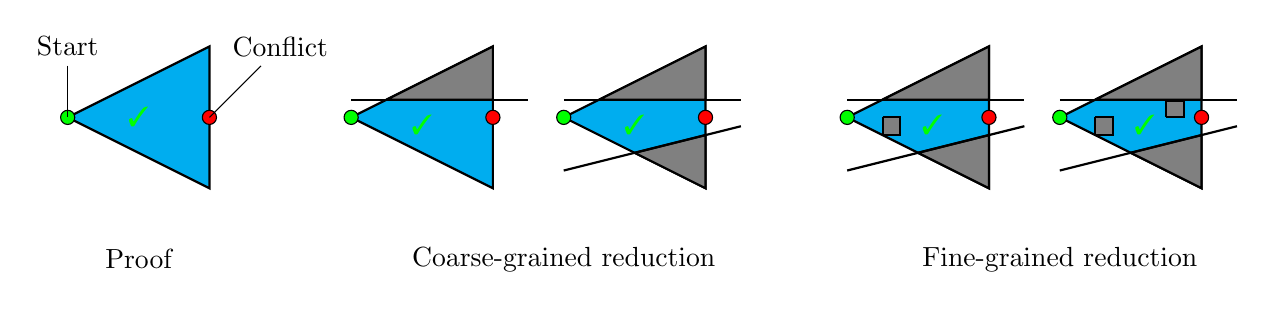
\begin{tikzpicture}[scale=0.9]

%\node at (-2,0) [rectangle,draw] (pre) {Delta-Debugging Image};

\draw [thick, fill=cyan] (0,0) -- (2,1) -- (2,-1) -- (0,0);
\draw [fill=red] (2,0) circle [radius=0.1];

\draw [fill=green] (0,0) circle [radius=0.1];

\node at (0,1) [rectangle]  (st) {Start};
\node at (3,1) [rectangle]  (cf) {Conflict};

\node at (1,0) [rectangle, green]  {\ding{51}};

\draw  (st) -- (0,0);
\draw (cf) -- (2,0);


\node at (1,-2) [rectangle]  {Proof};

\draw [thick, fill=cyan] (4,0) -- (6,1) -- (6,-1) -- (4,0);

\draw [thick, fill=gray]  (4.5,0.25) -- (6,0.25) -- (6,1) -- (4.5,0.25);
\draw [thick] (4,0.25) -- (6.5,0.25);

\draw [fill=red] (6,0) circle [radius=0.1];

\draw [fill=green] (4,0) circle [radius=0.1];

\node at (5,-0.1) [rectangle, green]  {\ding{51}};




\draw [thick, fill=cyan] (7,0) -- (9,1) -- (9,-1) -- (7,0);

\draw [thick, fill=gray]  (7.5,0.25) -- (9,0.25) -- (9,1) -- (7.5,0.25);
\draw [thick] (7,0.25) -- (9.5,0.25);

\draw [thick, fill=gray]  (8,-0.5) -- (9,-0.25) -- (9,-1) -- (8,-0.5);
\draw [thick] (7,-0.75) -- (9.5,-.125);

\draw [fill=red] (9,0) circle [radius=0.1];

\draw [fill=green] (7,0) circle [radius=0.1];

\node at (8,-0.1) [rectangle, green]  {\ding{51}};


\node at (7,-2) [rectangle]  {Coarse-grained reduction};


\draw [thick, fill=cyan] (11,0) -- (13,1) -- (13,-1) -- (11,0);

\draw [thick, fill=gray]  (11.5,0.25) -- (13,0.25) -- (13,1) -- (11.5,0.25);
\draw [thick] (11,0.25) -- (13.5,0.25);

\draw [thick, fill=gray]  (12,-0.5) -- (13,-0.25) -- (13,-1) -- (12,-0.5);
\draw [thick] (11,-0.75) -- (13.5,-.125);

\draw [thick, fill=gray]  (11.5,0) -- (11.75,0) -- (11.75,-0.25) -- (11.5,-0.25 ) -- (11.5,0) ;

\draw [fill=red] (13,0) circle [radius=0.1];

\draw [fill=green] (11,0) circle [radius=0.1];

\node at (12.2,-0.1) [rectangle, green]  {\ding{51}};





\draw [thick, fill=cyan] (14,0) -- (16,1) -- (16,-1) -- (14,0);

\draw [thick, fill=gray]  (14.5,0.25) -- (16,0.25) -- (16,1) -- (14.5,0.25);
\draw [thick] (14,0.25) -- (16.5,0.25);

\draw [thick, fill=gray]  (15,-0.5) -- (16,-0.25) -- (16,-1) -- (15,-0.5);
\draw [thick] (14,-0.75) -- (16.5,-.125);

\draw [thick, fill=gray]  (14.5,0) -- (14.75,0) -- (14.75,-0.25) -- (14.5,-0.25 ) -- (14.5,0) ;

\draw [thick, fill=gray]  (15.5,0) -- (15.75,0) -- (15.75,0.23) -- (15.5,0.23 ) -- (15.5,0) ;

\draw [fill=red] (16,0) circle [radius=0.1];

\draw [fill=green] (14,0) circle [radius=0.1];

\node at (15.2,-0.1) [rectangle, green]  {\ding{51}};

\node at (14,-2) [rectangle]  {Fine-grained reduction};

\end{tikzpicture}
\caption{Delta-debugging minimization of a proof, with a checkmark signifying the highlighted portion of the proof was verified by an independent proof checker.}
\label{fig:ddebug}
\vspace{-10pt}
\end{figure}
\fi

\newpage

\bibliographystyle{plain}
\bibliography{cattack}

\end{document}
